\documentclass{article}


\usepackage{arxiv}

\usepackage[utf8]{inputenc} % allow utf-8 input
\usepackage[T1]{fontenc}    % use 8-bit T1 fonts
\usepackage{hyperref}       % hyperlinks
\usepackage{url}            % simple URL typesetting
\usepackage{booktabs}       % professional-quality tables
\usepackage{amsfonts}       % blackboard math symbols
\usepackage{nicefrac}       % compact symbols for 1/2, etc.
\usepackage{microtype}      % microtypography
\usepackage{multirow}  % and items that fill up multiple rows in tables
\usepackage{graphicx}
\usepackage{xcolor,colortbl} % to add table color
\graphicspath{ {./images/} } % path to images
\usepackage{array} % add verticle space to tables

\title{Are we measuring what we think we are? Motivations and challenges of measuring the usage and impact of software designed for biomedical research}


\author{
Spyridon Bakas \\
    University of Pennsylvania \\
    Philadelphia, PA 19104 \\
    \texttt{sbakas@upenn.edu} \\
\AND
David Hanauer \\
    University of Michigan Medical School\\
    University of Michigan School of Information\\
    Ann Arbor, MI 48109\\
    \texttt{hanauer@umich.edu}
\AND
Carrie Wright \\
    Fred Hutchinson Cancer Center
    Seattle, WA 98109 \\
    \texttt{cwright2@fredhutch.org}\\
  %% \AND
  %% Coauthor \\
  %% Affiliation \\
  %% Address \\
  %% \texttt{email} \\
  %% \And
  %% Coauthor \\
  %% Affiliation \\
  %% Address \\
  %% \texttt{email} \\
}


\begin{document}
\maketitle
\begin{abstract}
Software has become vital in the advancement of biology and medicine. Analysis of usage and impact metrics of such software can be very beneficial to determining user and community contributor engagement. Such knowledge can be useful in justifying additional funding, encouraging additional use, and identifying unexpected usage. Furthermore, it can help define improvement areas and assist with managing project resources. However, there are several challenges associated with assessing usage and impact, many of which vary widely depending on the type of software being evaluated. These challenges involve issues of distorted, exaggerated, understated, or misleading metrics, as well as ethical and security concerns.  More attention to the nuances, challenges, and considerations involved in capturing impact across the diverse spectrum of biological software is needed. Although there are principles that can be generally applicable, there is not a single metric or approach to effectively evaluate a software tool’s impact, as this depends on aspects of the tool, how it is used, and how one wishes to evaluate engagement. We propose generalizable guidelines, as well as strategies for various types of software and resources. We also highlight outstanding issues in the field regarding how we measure or evaluate software impact. To gain an understanding of the issues hindering such evaluations, as well as to determine what appears to be helpful, we performed a survey of participants involved with scientific software projects for the Informatics Technology for Cancer Research (ITCR) program funded by the National Cancer Institute (NCI). We also performed investigations of software among this scientific community and others to determine how often infrastructure that supports such evaluations is implemented.  Our findings can help scientific software developers make the most out of the evaluations of their software so that they can more fully reap the benefits of such assessments.
\end{abstract}


% keywords can be removed
%\keywords{First keyword \and Second keyword \and More}


\section{Introduction} Biomedical software is critical to the advancement of biomedical research. The field has embraced and continues to embrace more open science practices, including the encouragement for sharing and harmonizing data and creating open source (publicly accessible and often freely available) software \cite{green_strategic_2020, levet_developing_2021, itcr_open-source_2021}. Often such open source software is initially developed so that the developers can use it themselves to reach a research goal \cite{bitzer_intrinsic_2007}. The software is then shared with the hopes that the use of the software by others will also contribute to the advancement of science or healthcare. Once shared, evaluations of the software is necessary to achieve two major benefits: 1) inform developers about how to improve the use and ultimately impact of the tool and 2) demonstrate the value of the tool to support the developers to obtain funding to continue to support existing software and to create new software. Common metrics include number of new users, returning users, and total usage of the software, but the type of metrics possible vary based on the type of tool and the context. These and other metrics, allow a project to gauge the rate of uptake of a project as well as how established it has become. However, developers often lack knowledge about the infrastructure or tools that can aid in the effective collection of usage and impact metrics. Proper metrics should not only examine the software's performance but assess whether motivations and goals of the researchers who are using the software are being met.

We aim to provide guidance for evaluations of software impact and engagement so that software developers can build tools that better meet researchers' needs to catalyze the progress of biomedical research. We will also discuss ethical considerations and challenges of such evaluations that still require solutions. The guidance presented here for software assessments holds the potential for developers to improve the use and utility of their tools, improve their chances of funding for future development, and ultimately lead to the development of even more useful software to advance science and medicine \cite{wratten_reproducible_2021}. 


\section{Overall guidance}





\subsection{Successful evaluations are anchored by an understanding of the intended use of the software}
\label{sec:use_understanding}
The intended goal or purpose of the scientific software should be used to inform how the software is evaluated. Computational tools are designed to support well-defined goals often called use cases \cite{gamma_design_1995} for specific sets of users called personas\cite{cooper_inmates_2004}. Efforts to evaluate the impact of tools should be guided by a clear understanding of these use cases and personas to assess how well the tools meet the intended goals.  

\subsection{Metric selection should be hypothesis driven} 
\label{sec:hypothesis_driven}
Collecting an exhaustive amount of user data, and then selecting metrics, can add complexity and increase the risk that metrics are selected in a biased manner. To mitigate this, metrics can be selected ahead of time based on a specific hypothesis to ultimately evaluate how well the software supports it’s intended goals. 


\subsection{Intentions for evaluation can also inform design choice} Software can also be designed with future evaluations in mind. Once the intended use of the software is clearly defined, avenues for what to investigate in terms of usage will also become clear. For example, Xena \cite{xena_2020} is a tool intended to enable users to visualize various aspects of the genome. The developers collect metrics involving how often users use the tool to perform  visualizations. However consideration of privacy led the developers to not collect metrics about what part of the genome gets visualized. 




\subsection{Metrics can achieve different goals for different audiences}

Clear understanding of which use cases, personas, and audience(s) are of interest, as well as what motivations are of interest, can help guide what user metrics to collect to achieve project goals.  For example, if the audience is the developers themselves, and the motivation is to learn how to retain new users, it may be helpful to understand how well new users are able to learn the basics of the tool. Thus focusing on metrics related to interactions with tutorials may be the most useful. These measurements might be very different from metrics used to understand which scripting features are being used by advanced users. 

It is also worthwhile to consider which presentations of software metrics will be most compelling to the intended audience. For example, detailed metrics on the inner workings of a software tool might be highly-informative to developers, but such metrics would be far too granular to be of interest to funding agencies. 
 


\subsubsection{Intrinsic motivations support tool optimization and development}

Tool optimization can involve improving workflows, performance, usage, or usability. 
Intrinsic motivations can also guide future work. For example, recognizing the types or volumes of data being used, as well as temporal trends of data usage, can highlight opportunities for new algorithm development. Similar analyses can help optimize resource allocation within and between projects. See Table \ref{tab:int_table} for more details.

\subsubsection{Extrinsic motivations seek to demonstrate tool value to gain external support}
 
 One of the most common extrinsic motivations is to provide evidence of tool impact to support requests for funding.  Evidence for impact is also often required to gain resources to develop or maintain semi- or un-related tools. Demonstration of past capability to develop impactful software supports requests to do so in the future.  Demonstrating that a tool is widely-used and widely-accepted can also encourage users to adopt a tool more readily, and be more invested in a tool community. Developers may be drawn to projects with impact to build upon an exiting tool. Finally, demonstration of impact can recruit new users which can diversify tool communities and bring new problems of interest that expand the utility of a tool.

\subsection{No single evaluation method works for every type of software}
\label{sec:no_one_way}
No individual scheme for collecting metrics fits every type of research software tool.  The meaning of a set of metrics may differ across different contexts. The location of a tool: whether it is on the web or locally downloaded can affect metric collection and influence user access to software versions. For example, for a web-based application, it may be feasible to collect user metrics on a per-account basis and to collect information about the type of data or software features users tend to work with. With this type of tool, users will rarely have access to older versions of the software. Thus developers can add version updates and collect metrics with clarity about how usage changed with updates. On the other hand, for tools that must be run (and possibly installed)  locally, users may be using older versions of the software that they previously downloaded.  Here, metrics on a per-version basis provide a much better representation of usage, rather than simply the overall number of unique downloads. Collection of version usage is important, as developers may want to pair this with citation data to know if users are using out-of-date aspects of previous versions of the software.


NOT SURE WHERE TO PUT THIS:
For example, you may find that your software is used widely in a country outside of the country in which you originally obtained funding to create that tool. Knowing this information, you could consider requesting funding for collaborators in that country to support that particular community.

 \subsection{Usage metrics assessments}
Once a project is generating sufficient user metrics, the next step is to interpret them to determine how they should inform the project's feature roadmap, development priorities, and outreach initiatives. This information can be used to estimate the level of "market penetration" that a tool has achieved. Although market share is difficult to estimate, it is important to have an expected community size and a measure of where a tool stands in comparison to its total potential use. It is also important to avoid comparisons between the community size and usage of tools with different approaches, i.e., between a desktop-based genome browser and a web-based repository of cancer data, given the different modes of use. 

When software has sufficient use, observed spikes in usage, both up and down, provide important feedback. A spike may correspond to a class or workshop that is given using the tool, a recent publication that cites the tool, or the unauthorized use of a resource. Negative trends in usage may indicate a break in the academic calendar, down time of a host server, or, for tools based on Amazon Web Services, the additional compute resources required by Amazon during holiday cycles may preempt software running on spot instances.


\subsection{Software infrastructure enables impact evaluation}
There are several components of a software tool that can assist with the assessments of the software impact and engagement. Once a developer team better understands their audience, use cases, personas, and assessment motivations, the following infrastructure could benefit or enable such evaluations, as well as improve user awareness and engagement. 

\subsubsection{Web presence}
Tools vary in terms of web presence. For example, some tools are web-based, some tools simply rely on a README file in a code repository, with simple installation information, while others provide extensive information and documentation on a separate website. Google Analytics can allow for more fine-grained tracking of how users are interacting with web-based tools or websites and can be helpful for later assessments, in addition to improving access, as one can also perform search engine optimization (SEO) to further encourage the visibility. For example, a developer could track what parts of the documentation users appear to read more frequently and pair this with information about common errors. For web-based tools, great detail can be determined about user interaction. Again Google Analytics can be helpful or for tools using a web-server manual log file inspection, or a service like Cronitor \cite{cronitor}  if the tool relies on a web-based server using cron \cite{cron_2009} job scheduling can also be informative.  It is however important to be mindful of user privacy regulations, see section \ref{sec:legal_ethics}.

\subsubsection{Citability}
Another component that can assist with evaluations is providing users with a method of citation, as well as information about how to cite the software, as some users may not be familiar with such practices. This is often done by publishing a manuscript about the software in a scientific journal and providing information about the publication on the software website and code repository. In addition, digital object identifiers (DOI), from publishing platforms like Zenodo, can be used for other less conventionally cited materials, such as documentation, case studies, data, and the actual software itself.

Services like Altmetric \cite{noauthor_altmetric_2015}, allow for deeper analysis of engagement for anything with a DOI. They provide reports and badges that can be added to websites or manuscripts (depending on where they are published) that indicate how often a DOI is cited in multiple sources besides scientific articles, such as blogs, news articles, Wikipedia, social media, and more.  Individuals or organizations can use Altmetric to get such reports by simply searching for the DOI. These reports also have links to individual social media posts, citing articles, and more. In addition, Semantic Scholar \cite{noauthor_semantic_nodate} provides reports that indicate where citations have occurred within scientific articles. 


\subsubsection{Documentation}
Documenting software not only helps guide users but can also enable collection of useful metrics.  Documentation on websites can be tracked and provide detailed information about such usage. If a particular page has more traffic, it may indicate that the aspect of the tool discussed on that page is either particularly popular or particularly confusing. As with all metrics, pairing information together can aid interpretation. Providing different types of documentation is another step that assures confidence in software, and enables varying roles to succeed in using the software. For example, command-line usage is important for the users of software, while API documentation is important for developers who may want to extend the software.

\subsubsection{Communications} 
Providing mechanisms for users to communicate with one another and with the developers can provide another avenue for understanding usage and engagement.

\subsubsubsection{Feedback mechanisms}

One very helpful method of obtaining software usage metrics is to have users directly provide feedback. Providing such feedback mechanisms helps to identify software weaknesses. However, few users provide feedback and often feedback requires interpretation. Individuals are also unlikely to provide positive feedback. Nevertheless, user feedback mechanisms can be powerful for gaining insight from users. 
Feedback mechanisms can be passive or active in nature. More passive mechanisms may involve providing an email address on a website or simply allowing users to post an issue on a GitHub repository. More active mechanisms may include usability testing interviews, Google forms or other surveys, or providing automated GitHub issue templates to encourage specific kinds of feedback.


\subsubsection{Email and support forums}
While it’s possible to collect user feedback and provide support through email,  if a public support forum is used instead, users can learn from answers to questions of other users, reducing the burden on developers, and provide another opportunity for easier tracking of software engagement. This also provides an opportunity to build a community around the software and to learn what is and isn’t working for users. Some forum platforms support upvoting (where other forum users can upvote questions or feature requests). Using an existing support forum platform such as Discourse (\url{https://www.discourse.org/}) provides many features that are convenient in forum moderation, such as user trust levels, categorization and tagging of topics, and detailed tracking of forum posts, forum post views, and user and moderator activity levels that serve as useful metrics about a software project and the community around it.

Engaging with users about what new features they are excited about and acting on those discussions, is a great way to get informed feedback while rewarding user involvement. To further support community, developers could consider inviting user to attend workshops on new features or inviting them to help teach workshops on fundamentals.  Forum members who provide intellectual contributions to projects, including technical support, feature suggestions, highly referenced posts, etc, should be included as authors on relevant papers. And public facing activity summaries (e.g., \url{https://forum.qiime2.org/u/gregcaporaso/summary}) can also be useful for resume building for early career contributors.

Emailing newsletters to registered users, can be a useful method for informing users about new features, updates or issues. Systems like Mailchimp \cite{mailchimp} or HubSpot \cite{hubspot} can allow analytics about how often recipients open the news letter, click on links, or unsubscribe.

\subsubsection{Usability testing}

Usability refers to the ease of use for an individual to use software. Usability testing is a method of purposefully investigating the usability of a software tool. Usability testing can be highly powerful for collecting valuable metrics and information regarding the usage. This involves applying the scientific method to investigating a user's experience with a software tool and asking users to use the software tool while the tester observes their interactions with the tool. 

Often research institutions do not have these experts in user design and testing on staff. However, developers can and should utilize these techniques to conduct their own informal usability testing. Step-by-step guides of how to conduct usability testing have been published elsewhere \cite{savonen_2021}.  It should be noted that the benefits of usability testing are high even when only a few users are observed. 

\subsubsection{Workshops}
Hands-on workshops (online\cite{dillon_experiences_2021} or in-person) for your software are an excellent way to build a user community and get feedback. Workshops allow developers identify what confuses or challenges users. This can be illuminating as the challenges are often not what developers expect. Attendees can also be asked to participate in surveys about what they like and don't like to help guide future development. The quantity, duration, and attendance at your workshops are metrics that can be reported to funding agencies in grant proposals or reports. Posting recordings of events can be shared on YouTube or other platforms, which allows for other useful metrics. 

\subsubsection{Code of conduct}
Before engaging with user or developer communities, it is important to develop and publish a code of conduct for your project to outline expectations of behavior and how contributors can report violations. A code of conduct can be reassuring of community health and are required by some scientific software funders, such as the Chan Zuckerberg Initative’s Essential Open Source Software for Science program. Thus the presence of a Code of Conduct may be a measure that is assessed by potential funders. A good starting point for a code of conduct is the Contributor Covenant (https://www.contributor-covenant.org/), which can be adapted. Adopting and effectively managing\cite{aurora_how_2019} a  Code of Conduct can support the growth of your community by indicating a safe space, thereby encouraging engagement by individuals who might feel intimidated about getting publicly involved.

\subsubsection{Social media}
Having a social media presence through platforms such as twitter, instagram, and youtube, provides opportunities to track engagement with social media posts.  Pairing this with evaluations of engagement with the software itself, to determine if outreach strategies are successful. This can also be helpful to determine if documentation resources are useful. For example, the number of video views on a youtube documentation video can be informative to know what percentage of users may have actually seen the documentation. Videos with many views can also reassure others about using the software . 

\subsection{Reviews}
There are review mechanisms that can help reassure users about software. For example, SourceForge\cite{sourceforge} a platform for publishing and developing software allows users to rate software on the platform. Developers can integrate their GitHub repositories with SorceForge to take advantage of this review platform. Alternatively, GitHub also has a system of adding stars or followers to repositories, however, this appears to be somewhat inconsistently done in the community. 

\subsection{Software project health metrics can reassure users and funders}
Tracking adherence to standards of software engineering can be a useful way to assess software project health including the use of version control systems, high coverage of code with testing, and use of automated or continuous integration. None of these measures of project health are perfect but can be collectively assessed as indicators of whether a project is healthy. Like any tool, version control and testing can be used well or poorly, and the appropriate use of these tools truly indicates project health. A good resource for additional detail on these topics, can be found in The Pragmatic Programmer\cite{thomas_pragmatic_2019}. 

\subsubsection{Version control mechanisms}
Many bioinformatics software projects maintain their source code under public revision or version control, using a platform such as GitHub or GitLab. Provided that the platform is actually used for version control (as opposed to hosting one or two versions of the software), this is a useful indicator of project health. Users can be confident that changes to the code are tracked to some extent and can also observe how much activity and updates have occurred to the software -- this can indicate to the user and developers fo the project how recently maintenance has occurred. This can also help users identify the specific version or revision of the software they are using to record and report their methods, reproduce an analysis, or determine if they are impacted by a bug in the software. Furthermore, GitHub provides an insight tab with information about development metrics and its API allows for collection of these metrics in a systematic and reproducible way. 

\subsection{Development activity}

Finally project health can be assessed based on activity. By reviewing the frequency of commits and the date of the most recent commit in a revision control system, it is possible to assess whether the project is actively developed. Inactively developed projects project may not include fixes for recently discovered bugs, or improvements in methods to keep current with the field. Tracking who is making commits to the project can also provide details on whether the project is the work of one or a few developers, or of a large and active developer community. Neither a big or small developer community is necessarily better, though smaller developer communities can pose greater sustainability risk. If there is only one person who knows how to work on the code, and that person becomes unable or unwilling to continue working on the project, development or maintenance of the project may be discontinued. 



\subsubsection{Automated test coverage and continuous integration testing}

Bugs in scientific software can have far-reaching impacts. Automated software tests allow developers to confirm that their code is behaving as expected under a range of normal and abnormal conditions. Systematically developed tests that can be run by both developers and users with a single command, give confidence that the software is doing what it is supposed to be doing. Platforms such as GitHub allow developers to advertise their test code coverage (the fraction of lines of code in the project that are covered by automated tests) and current build status (including whether tests are currently passing or failing). The presence or absence of this information, as well as quantitative metrics like test code coverage, are useful indicators of project health. Similarly, the use of automated or continuous integration testing, which can be configured to run when a change is committed to a software repository, when software releases are created, or at any other point where quality assurance is necessary to provide early signals of errors, is also an indicator of project health. This can help ensure that bugs or other issues can be detected before software is deployed by users.

The presence of different types of automated tests can be seen as an indicator of software maturity, and the care taken in the process of developing the software. Unit tests provide confidence in individual pieces of code; component and integration tests provide confidence that individual pieces of code behave correctly together; acceptance tests provide confidence that the overall software behaviors are correct. Achieving this in-depth test coverage requires careful software design upfront and throughout development. It is worth noting that, while useful, test coverage is not always a trustworthy representation of test quality. It is simply a measure of the proportion of code which is run by the test suite. It does not evaluate the quality of the test cases or assertions.

Other related static code analysis metrics can be used in conjunction with test coverage to build a more well-rounded picture of code quality. For example, cyclomatic complexity measures the logical complexity of a function. Code with high cyclomatic complexity contains numerous branching paths with variations in execution, and therefore should be avoided. It’s clear that a complex function can have 100\% test coverage without coming close to testing all possible outcomes. In fact, writing tests for highly complex code is often a lost cause. By considering cyclomatic complexity alongside test coverage, programmers can target specific areas of a codebase that need more tests. However, they can also see where they should instead prioritize refactoring, reducing complexity and improving testability first.

\subsubsection{Licensing}
In general, a software project should have a discoverable license that allows users to understand how they are and are not allowed to use the software. Licenses differ in how permissive they are, but the lack of a license defaults to highly restrictive terms and is an indicator that use of the software by others hasn’t been adequately considered. Similarly, the choice of license can be another indicator of inadequate usage consideration due to the restrictive and binding nature of some software licenses. 



\section{Operationalization}

Operationalization is the process of defining quantitative metrics for phenomena that are not explicitly measurable, to move them from abstract concepts to quantitatively measurable variables. In relation to software user metrics, this often involves defining a desired goal for engagement with the software and describing which specific, observable events, variables or behaviors can be considered to reflect that. This enables testing of hypotheses about this aspect of the software, at which point efforts can be made to improve the software in response, measuring success via the measurement of those variables. 

Careful consideration of the use case can provide a good starting point. In a simple case, we might account the total unique downloads as a metric of our software’s popularity, but this only reflects how many people have tried to download it and not if users find it useful. If we want information on how often users use our software, we might count the number of launches of the software which run over a certain predefined session time threshold, or after the user completes a tutorial. If we want our tool to support the majority of data in the field, we might collect instance counts of each data type users attempt to load with the tool. Even with limited data, such as that provided by in-house testing, specific quantitative measures provide a common basis for the interpretation of software metrics. In this way, the software can be compared between versions and potentially against other similar software. Only once these distinct variables have been identified can their collection be implemented using either pre- or custom-built solutions.

\section{Challenges and nuances}

\subsection{Citation challenges}
Measuring the number of citations of your tool is important, especially as a metric to report to funding agencies. First, it is important that your tool has a manuscript or other data object to cite \cite{chue_hong_software_2019}. While publishing a manuscript in a formal publication is often the ultimate goal for a tool, having a manuscript published as a preprint such as BioRxiv, or even in Figshare (see the example The graph-tool python library \cite{peixoto_graph-tool_2017}), can help a tool to have a citable presence. For data objects, Zenodo and Data Dryad can provide DOIs, which are citable. Note that having a pre-final published version of your tool may make it difficult to track citations in the future once a manuscript is formally published as tool developers will have to follow citations for both publications.

Once a tool is published, getting users to cite a tool or cite it correctly can be difficult. First, some tools are so common that users often don't think to cite them, similar to how a scientist would not cite Microsoft Word when writing a publication, despite the crucial role Microsoft Word played in the writing process. An example of a tool like this would be the UCSC Genome Browser. Second, some tools are used in the discovery phase of a project, and a user may not think of it when they are in the final stages of writing up findings. An example would be a tool used to find a discovery cohort of patients such as EMERSE (Electronic Medical Record Search Engine). Third, tools which provide system architecture for a other software may also not be typically cited. Some tools in this category include Bioconductor, Gene Pattern Notebook, and Galaxy. understanding citations may require looking at usage of other tools that are available on these platforms. Lastly, while users may recognize and acknowledge your tool, they may not cite the tool in the reference section of their paper and they may mention the tool without complete information, such as not including version information, parameter settings, URLs, or credit to those who made the software.  In fact, a study manually evaluating software citations of 4,971 academic biomedical and economics articles, found that the citations only included version information  28\% of the time \cite{howison_software_2016}.  Another study manually evaluating 90 biology articles, also finds a low rate of complete information with version information being included only 27\% of the time and URL information included only 17\% of the time \cite{du_softcite_2021}. People may  mentioning a tool in a figure legend, in the paper itself, in the acknowledgments, or even in the abstract, without a citation. These mentions of a tool are difficult to track. Furthermore, occasionally manuscripts simply acknowledge that a software tool exists, rather than indicating that it was actually used by the authors. In other cases a newer version of a tool is used, yet a previous publication for an earlier version of the tool may often be cited by these users. This typically requires manually reading articles. 

Fortunately, there are a number of tools that can help you measure citations. These include Google Scholar, Web of Science, PubMed, and ResearchGate. Additionally, some tools are being developed to help track software mentions, such as the tool CORD-19 Software Mentions \cite{wade_cord-19_2021}. Each of these citation measuring tools also have options to help overcome the difficulties mentioned above. For instance, Google Scholar and PubMed will allow you to search for the name of a tool anywhere in a paper. In addition Semantic Scholar allows for reports of where citations are located across papers. Note that tools names that alias with other terms, such as Galaxy, can make it more difficult to use these options to find additional citations. A couple of recent papers \cite{istrate_large_2022, schindler_role_2022} have also developed automated extraction methods to overcome additional challenges, such as disambiguating multiple synonyms for the same software, typos or misspelling, the use of acronyms vs full names, and deeper capture of version information. 

It is also important to note that if other software relies on your software, it is likely useful to evaluate the citations of other such software in your analysis of the impact of your software. However, it can be difficult to know if this software exists if the developers do not adequately describe dependencies in a manuscript or documentation.

\subsection{Limitations of tracking systems}
One other difficulty with the implementation analytics platforms such as Google Analytics. Due to security and privacy concerns, we note that some academic institutions are blocking connections to these services outright. Other, unknown or custom-built tracking may be flagged by security software or otherwise generically blocked. Hence, reliance on this data may not paint the full picture of industrial or academic usage, especially if interest is concentrated in one of these institutions.

\subsection{Distorted metrics}

Projects like Bioconductor, which have a large number of different software packages, can get a greater sense of how different packages compare and are used over time. This can reveal important nuances. One interesting finding is that occasionally scripts used on servers may download a package repeatedly and rapidly on accident hundreds to thousands of times. Since this does not indicate real usage likely beyond one user, this can result in distorted download metrics. Therefore, unique IP download information, is useful to determine if usage represents one user many times versus many users a few times. Given privacy concerns, a alternative solution could be tracking the timing and general location of downloads with a threshold for what might be more than a group of people following a tutorial to identify such scripts. It was also found that there is a baseline background level of downloads across all packages (including those that are no longer supported). Thus a new package may have 250 downloads in the first year year. While out of context this may seem like a successful number, looking at other packages, it can be determined that this is more similar to background levels. Another example, is the S4Vectors package which is an infrastructure package used by many other packages mostly for technical and non-biological reasons and is therefore not often directly downloaded by end-users. This package is also used for automated checks for bioconductor packages more generally using GitHub actions, therefore, it can be difficult to discern if the usage of a package is for scientific research itself or supporting the development of other software. While both are arguably very valuable, distinguishing between these motivations can help us understand a particular software's impact in a field.  Another interesting example is the affy package \cite{affy} , which was one of the early Bioconductor packages for microarray analysis, a technology that has largely been replaced by newer technologies. However, despite a clear transition by the field away from microarray \cite{mantione_comparing_2014}, The affy package was downloaded in 2021 at rates that doubled the rates on 2011. It is believed that this is due to people historically requesting that it be installed on servers and that this is just persisting. Another situation in which metrics such as "registered" users may be distorted, is when a single instance of software is registered for an institution and then a provisioning system allows use for multiple users through for example virtual machines. 


background IP downloads, automated checks, infrastructure package used by other packages, older packages will have more downloads, 



Usage as an (imperfect) proxy for maturity

\subsection{Tracking with cloud environments}
Tracking usage in a cloud-driven vs. other more conventional environment (ie. users are running software on dnanexus, terra, etc.)



\subsection{Clinical data challenges}

Systems that contain clinical data have unique challenges.  Clinical data (generally defined as those data extracted from electronic health record systems) are often comprised of highly sensitive protected health information (PHI), which means that the scope of users with access is quite limited. Thus, while the clinical details can be vital for research, the number of individuals that have access to the data is generally much smaller than tools designed to work with non-clinical data. Clinical research teams can be constrained by their health system on what type of computer systems software can be installed on. Many tools containing clinical data are also run at an enterprise level, meaning that they are installed only one time, centrally, by system administrators with accounts provisioned to users. This affords sites greater control over the access to restricted PHI and the necessary auditing functions needed to record viewing patient information, and helps prevent the egress of PHI by reducing the number of copies of the data distributed to end users.  However, such a scenario means that counting installations does not represent the overall use of the system, and it is not common for system administrators to send usage reports externally to software development teams interested in tracking usage.  Further, the firewalls protecting these systems, as well as the built in security, precludes developers from accessing the installed systems themselves. Other approaches, such as software “phoning home” could raise flags by security teams looking for unusual behavior, especially malicious software that could be trying to send clinical data outside of the covered entity. Our experience within the EMERSE team is that even the GitHub page for our open source software is now in a private repository. This was done for two reasons: (1) we can better understand who are interested implementers are by inviting them to the repository and developing a relationship with them and (2) our health system security team preferred this approach to let only known entities access the software in order to prevent those with malicious intentions from looking for vulnerabilities that may have been missed despite rigorous, continuous security reviews.  It is worth noting that because our software is open source others could post copies of the code in other open repositories that we do not control.  However, since we all share a common goal of heightened security, no group has yet done this to the best of our knowledge. Ultimately due to downloads typically being at an institutional level for clinical tools, metrics around software downloads, would underestimate the potential impact of clinical tools. Funding agencies need to consider how each type of tool is context dependent and that impact should be measured and compared between tools with this in mind.  

\section{Software fairness evaluation}



\section{Goodhart’s law}
An important consideration for any metrics that are used to assess a tool is Goodhart’s Law, which states that “every measure which becomes a target becomes a bad measure\cite{hoskin_awful_1996}”. As an example, h-indices are often used to assess the quality of an author’s impact. However, as the h-index (i.e., the number of papers an author has with that many or more citations) grew in popularity, the number of researchers included as co-authors, the number of citations per paper, and the fraction of self-citations increased. Each of these would lead to an increased h-index. At the same time, these behaviors would also increase a journal’s impact factor \cite{fire_over-optimization_2019}. Altmetric, which we described earlier may help in providing more information about more diverse engagements with articles (social media, news), however it does less to aid in evaluating author contribution. It is not a stretch to imagine that as metrics are developed and codified for tools would lead to developers attempts to improve the metric for their tool. Although Goodhart’s Law could be used to bring about best practices for binary outcomes (i.e., compliance with codes of conduct, public deposition of code), for more quantitative metrics (e.g., number of downloads, citations) the results would easily render the metrics meaningless. One way to avoid this, is to continue to evaluate our metrics overtime, consider if our metrics are truly measuring what we think they are, consider if our metrics are actually fair to a diverse range of people, and consider newer more nuanced metrics \cite{fire_over-optimization_2019}. One example of such unfairness would be evaluations of metrics for clinical data resources that are inherently limited in terms of who can be allowed to access the resource. Such caveats need to be accounted for when evaluating and comparing tools and resources.

\section{Security, legal, and ethical considerations}

\subsection{Security}
In any repository that contains source code, it is of vital importance that authentication secrets, such as API keys or cryptographic secrets be managed properly \cite{merkel_docker_nodate}. It becomes even more important in the case of code that deals with healthcare data, where even the slightest mishap in this regard could potentially expose protected health information (PHI) data and/or information to the public. During the continuous integration (CI) step of any project, incorporation of reputed static code analysis tools \cite{louridas_static_2006, ludwig_compiling_2017} (which are often available to open-source projects at no cost) ensures that tracking of the perpetually evolving landscape of security threats is offloaded to an entity that is specialized for its detection. It also allows the code to scale at a quick pace while ensuring bugs can be identified early in the development process, and finally allows software architects to define security guidelines to assist developers without impeding on their development process.
It is understood and accepted that open-source code is built “on the shoulders of others”, and regular analysis of the underlying dependencies (such as using the “Dependabot” product from GitHub \cite{noauthor_dependabot_nodate}) allows the automatic detection of security vulnerabilities (and potential mitigation strategies presented) to the development team in question \cite{alfadel_use_2021}. Products such as Dependabot maintain a frequently updated collection of packages with version/commit identifiers that contain security vulnerabilities with their fixes as defined by the broader community, and as such should be incorporated into all open-source repositories. Another set of security considerations come when packaging and deploying code in the form of containers, and more specifically using Dockers \cite{merkel_docker_nodate}. Depending on the veracity of the adversary in question, attacks on Docker containers can range from targeting the container itself, the host system, any collocated containers, the container management system or the source code itself\cite{combe_docker_2016}. One of the most common security threats from Docker containers come in the form of elevated user access \cite{combe_docker_2016, bui_analysis_2015}, which can be a critical flaw when running containers in an High Performance Computing (HPC) environment \cite{sparks_enabling_2019, bacis_dockerpolicymodules_2015}. This is specifically addressed using other containerization protocols such Singularity \cite{kurtzer_singularity_2017} and Podman \cite{gantikow_rootless_2020}. Though a single solution might not work for all cases, when deploying open-source software using the Docker containerization protocol, specific security mitigation strategies should be considered \cite{yasrab_mitigating_2021}.

\subsection{Legal and ethical considerations}\label{sec:legal_ethics}
Often with the use of phone home or web-based analytics, users are tracked for not only downloads, but often for specific elements of usage, such as the number of times users open a desktop application that relies on an external server, the number of times a user runs a particular kind of analysis, etc. Occasionally software developers will notify users that they are being tracked, however this is often not a requirement. The General Data Protection Regulation (GDPR) which became implemented in 2018, requires that organizations anywhere in the world respect certain data collection obligations regarding people in the European Union. It is intended to protect the data privacy of individuals and mostly guards against the collection of identifiable personal information. Thus data collection of software usage, needs to be mindful of the GDPR and any other international regulations that may impact data collection of users.  As science is particularly an international pursuit, often a majority of the users may reside outside the country where the tool was developed.

One option is to let users determine if they wish to be tracked by letting them know during certain stages of use depending on the type of software, such as when users download, register, or use certain features 
 of software. It is also possible for software developers to design tracking to be more anonymous, for example a genome visualization tool may track the number of unique uses, but it will not track what part of the genome was visualized. Google Analytics also provides support for how to comply with such restrictions, for example you can  mask unique IP addresses of visitors to a website that tracked by the system \cite{google_analytics_privacy}.  Ethical and legal consequences should be considered when designing or implementing tracking systems of scientific software. 



\section{Discussion and conclusion:}
 Ideas about improvements to encouraging more metric analysis, transparency, metric collection, overcoming challenges, and ethical considerations. Possible discussion of future outlook.
\subsection{Figures}

See Figure \ref{fig:altmetric}.

\begin{figure} % picture
    \centering
    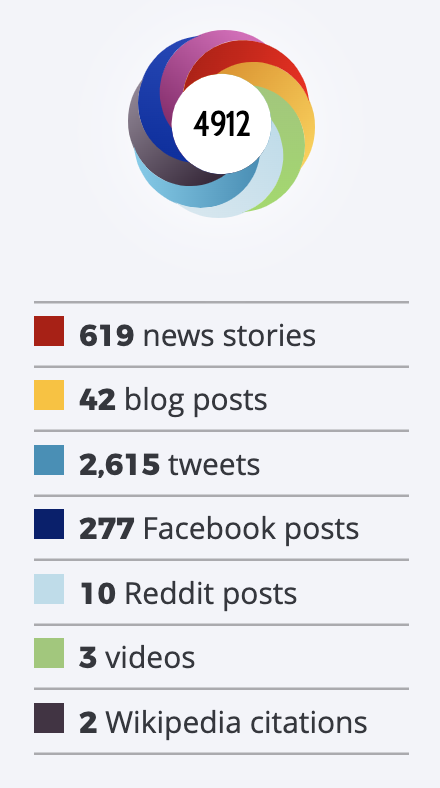
\includegraphics{altmetric.png}
    \caption{Example of an Altmetric Summary from \url{https://www.altmetric.com/top100/2016/}}
    \label{fig:altmetric}
\end{figure}

\subsection{Tables}

See awesome Table~\ref{tab:int_table} Table~\ref{tab:ext_table} and Table ~\ref{tab:opt_table}.
\renewcommand{\arraystretch}{1.1} %adding space between rows will influence the rest of the document

\begin{table}
 \caption{Extrinsic Motivations}
  \centering
  \begin{tabular}{|l|c|p{0.3 \linewidth}|}
    \hline
    \multicolumn{1}{|c|}{\cellcolor[gray]{.9} \textbf{General Goal}} 
    & \multicolumn{1}{|c|}{\cellcolor[gray]{.9} \textbf{Specific Goal}}
    & \multicolumn{1}{|c|}{\cellcolor[gray]{.9} \textbf{Task}}\\[1.1ex] % add some space after headers before horizontal line
    \hline
    \multirow{4}{*}{Gaining Support}              
    & \multirow{4}{*}{Evidence of Impact} & 
    Supporting future funding requests \\
    & &
    (to maintain or develop new tools) \\
    & &
    Requesting for resources  \\
    & & 
    (to maintain or develop new tools) \\[1.1ex]
    \hline
    \multirow{4}{*}{ Commitment of users} 
    & \multirow{4}{*}{Evidence of tool acceptance} & 
    Reassuring users about tool to:\\
    &&
    - Promote continued use\\
    && 
    - Promote usage of new tools by the same developers \\ 
    &&
    - Promote usage by more diverse users \\[1.1ex]
    \hline
    \multirow{1}{*}{Commitment of community developers} 
    & \multirow{1}{*}{Evidence of co-development} & 
    Encouraging contributions by other developers \\
    \hline
  \end{tabular}
  \label{tab:ext_table}
\end{table}


\begin{table}
 \caption{Intrinsic Motivations}
  \centering
  \begin{tabular}{|c|c|l|}
    \hline
    \multicolumn{1}{|c|}{\cellcolor[gray]{.9} \textbf{General Goal}} 
    & \multicolumn{1}{|c|}{\cellcolor[gray]{.9} \textbf{Specific Goal}}
    & \multicolumn{1}{|c|}{\cellcolor[gray]{.9} \textbf{Task}}\\
    \hline
    \multirow{17}{*}{Tool Optimization}               
    & \multirow{3}{*}{Improving Workflows} & 
    Identifying unexpected usage \\
    & &
    Identifying inefficiencies \\
    & &
    Identifying inadequate documentation\\ \cline{2-3}
    &   \multirow{4}{*}{  }
    & 
     Identifying mismatches with defaults and use \\
     &  Improving Performance  &
     Identifying errors \\
    &  &
    Assessing run-time \\
    &  & 
     Measuring data volume \\  \cline{2-3}
    & \multirow{5}{*}{ Improving Usage} & 
    Identifying who the user-base is \\
    & &
    Determining user-base diversity \\
    & &
    Identifying sources of other possible users \\
    & &
    Determining what users expectations are \\
    & &
    Determining if user expectations are appropriate \\
    & &
    Evaluating success of outreach approaches\\  \cline{2-3}
    & \multirow{2}{*}{ Improving Implementation} & 
    Identifying barriers for adaption \\
    &   &
    Identifying methods to support adaption \\
    &  & 
    Identifying use of out-dated versions\\\cline{2-3}
    & \multirow{2}{*}{ Improving Usability} & 
    Identifying what features are used \\
    & & 
    Identifying which users use which features \\
    &  &
    Identifying what features are not being used \\
    & &
    Identify if and how users are struggling \\ 
    \hline
    \multirow{6}{*}{\shortstack{Tool Development \\ \& Maintenance}}
    & \multirow{6}{*}{\shortstack{ Guiding Future Work\\  Motivating Continued Support}} &
    Enumerating data types being used \\
    & &
    Measuring volume of data use \\
    & &
    Discovering opportunities for new features \\
    && 
    Discovering data needed to address user goals  \\
    & & 
    Identifying more appropriate resource allocation \\
    & & 
    Identifying strategies to reduce barriers \\
    \hline
  \end{tabular}
  \label{tab:int_table}
\end{table}


\begin{table}
 \caption{Operationalization}
  \centering
  \begin{tabular}{|c|l|l|}
    \hline
    \multicolumn{1}{|c|} {\cellcolor[gray]{.9} \textbf{Measure}}   
    & \multicolumn{1}{|c|} {\cellcolor[gray]{.9} \textbf{Example Metrics}}     
    & \multicolumn{1}{|c|} {\cellcolor[gray]{.9} \textbf{Use}}  \\
    \hline
    Tool dissemination & 
    Total unique downloads & 
    Popularity of a given tool \\
    & 
    Download count by version &
    Users keeping up-to-date\\
    \hline
    Tool usefulness & 
    Average run count, by user & 
    Determining prevalence of usage \\
    \hline
    Tool reliability & 
    Proportion of runs without a crash or error &
    Improving error handling, bug fixes\\
    \hline
    Tool versatility &
    Distribution of data types (inferred from metadata)&
    Improving tool flexibility\\
    Interface acceptability &
    Average user session length &
    Graphical tool and website acceptability\\
    \hline
    Performance &
    Maximum memory usage &
    Tuning, requirements analysis\\
    &
    Average time-to-complete of algorithmic steps &
    Tuning,
    requirements analysis \\
    \hline
  \end{tabular}
  \label{tab:opt_table}
\end{table}

 
\bibliographystyle{unsrt} 

\bibliography{references}


\end{document}
